\documentclass{article}
\usepackage{amsmath}
\usepackage{tikz}
\usepackage{pgfplots}
\pgfplotsset{compat=1.18}
\usepackage[a4paper, margin=2cm]{geometry}

\begin{document}

\title{函數圖形生成器測試文檔}
\author{FunctionPlotGenerator}
\date{\today}
\maketitle

\section*{測試目的}
本文檔測試 FunctionPlotGenerator 生成器的四種函數類型:
\begin{itemize}
  \item 多項式函數 (Polynomial)
  \item 指數函數 (Exponential)
  \item 對數函數 (Logarithmic)
  \item 三角函數 (Trigonometric)
\end{itemize}

\newpage

\section*{1. 多項式函數: $f(x) = x^2 - 2x + 1$}

\begin{center}
% 函數圖形
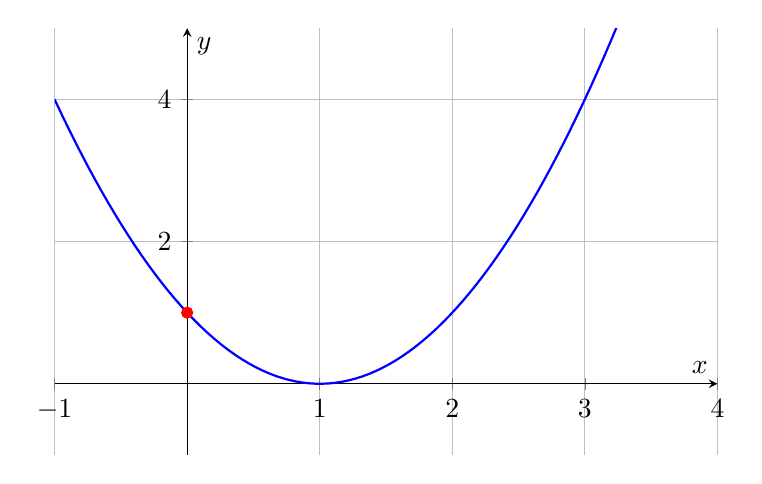
\begin{tikzpicture}
  \begin{axis}[xmin=-1, xmax=4, ymin=-1, ymax=5, axis lines=middle, width=10cm, height=7cm, grid=major, xlabel=$x$, ylabel=$y$]
    \addplot[blue, thick, domain=-1:4, samples=100] {x^2 - 2*x + 1};
    \addplot[red, only marks, mark=*] coordinates {(0, 1)};
  \end{axis}
\end{tikzpicture}
\end{center}

\vspace{1cm}

\section*{2. 指數函數: $f(x) = 2^x$}

\begin{center}
% 函數圖形
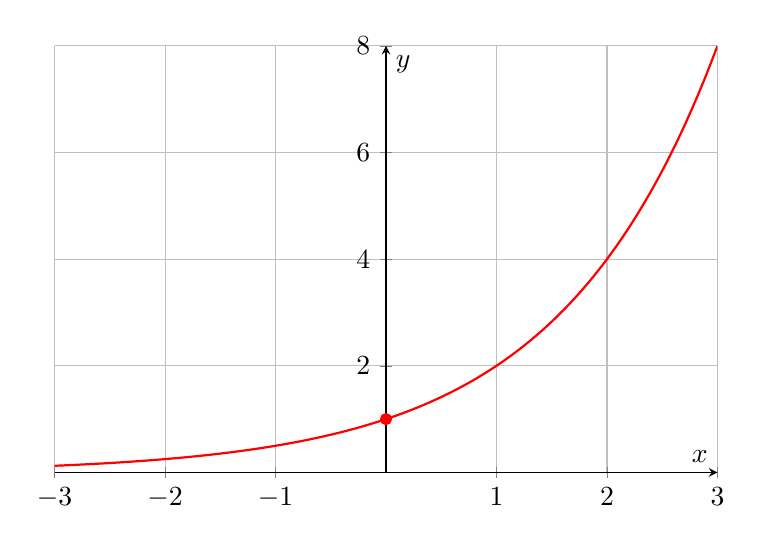
\begin{tikzpicture}
  \begin{axis}[xmin=-3, xmax=3, ymin=0, ymax=8, axis lines=middle, width=10cm, height=7cm, grid=major, xlabel=$x$, ylabel=$y$]
    \addplot[red, thick, domain=-3:3, samples=100] {2.0^x};
    \addplot[red, only marks, mark=*] coordinates {(0, 1)};
  \end{axis}
\end{tikzpicture}
\end{center}

\vspace{1cm}

\section*{3. 對數函數: $f(x) = \log_2(x)$}

\begin{center}
% 函數圖形
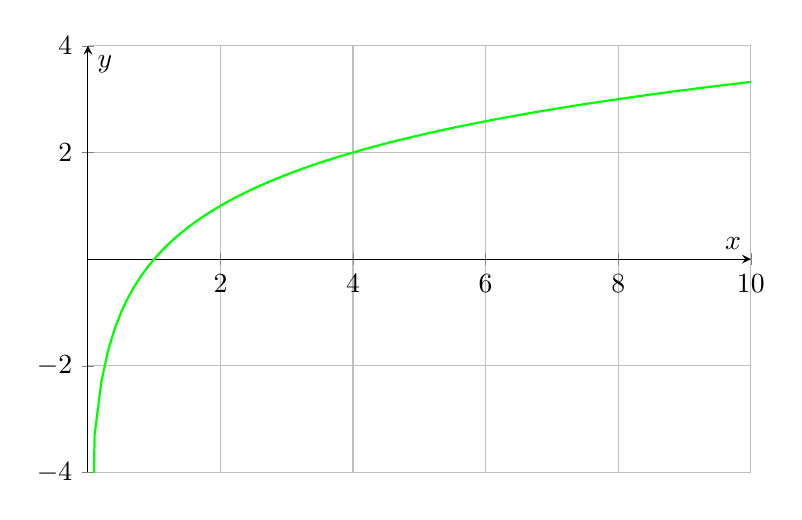
\begin{tikzpicture}
  \begin{axis}[xmin=0.001, xmax=10, ymin=-4, ymax=4, axis lines=middle, width=10cm, height=7cm, grid=major, xlabel=$x$, ylabel=$y$]
    \addplot[green, thick, domain=0.001:10, samples=100] {ln(x)/ln(2.0)};
  \end{axis}
\end{tikzpicture}
\end{center}

\vspace{1cm}

\section*{4. 三角函數: $f(x) = 2\sin(x)$}

\begin{center}
% 函數圖形
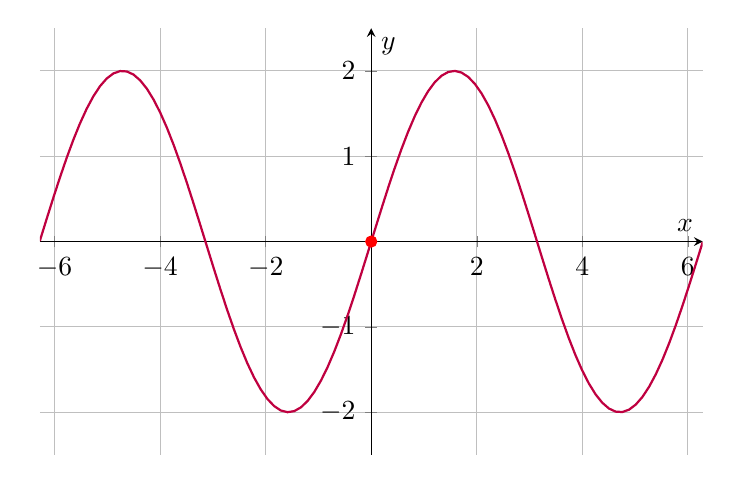
\begin{tikzpicture}
  \begin{axis}[xmin=-6.28, xmax=6.28, ymin=-2.5, ymax=2.5, axis lines=middle, width=10cm, height=7cm, grid=major, xlabel=$x$, ylabel=$y$, trig format=rad]
    \addplot[purple, thick, domain=-6.28:6.28, samples=100] {2*sin(x)};
    \addplot[red, only marks, mark=*] coordinates {(0, 0)};
  \end{axis}
\end{tikzpicture}
\end{center}

\vspace{1cm}

\section*{5. 三角函數: $f(x) = \cos(x)$}

\begin{center}
% 函數圖形
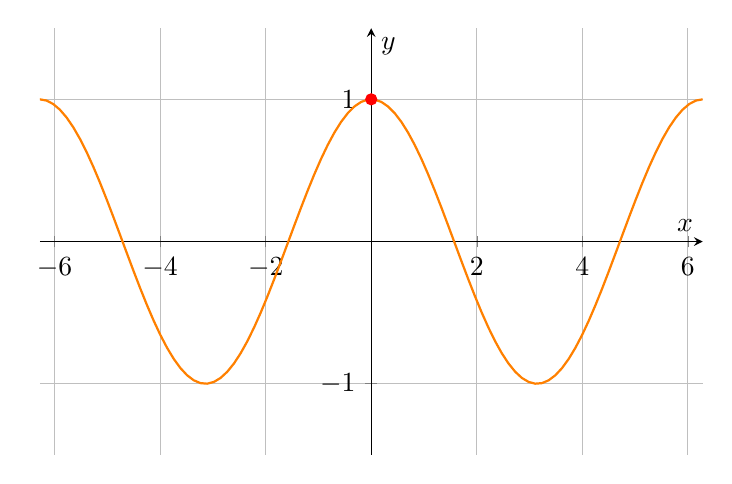
\begin{tikzpicture}
  \begin{axis}[xmin=-6.28, xmax=6.28, ymin=-1.5, ymax=1.5, axis lines=middle, width=10cm, height=7cm, grid=major, xlabel=$x$, ylabel=$y$, trig format=rad]
    \addplot[orange, thick, domain=-6.28:6.28, samples=100] {cos(x)};
    \addplot[red, only marks, mark=*] coordinates {(0, 1)};
  \end{axis}
\end{tikzpicture}
\end{center}

\vspace{1cm}

\section*{6. 三角函數: $f(x) = \tan(x)$ (自動處理不連續)}

\begin{center}
% 函數圖形
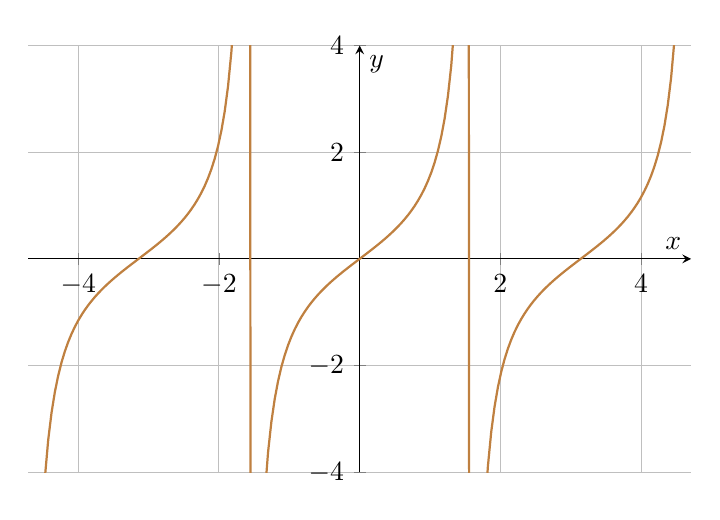
\begin{tikzpicture}
  \begin{axis}[xmin=-4.71, xmax=4.71, ymin=-4, ymax=4, axis lines=middle, width=10cm, height=7cm, grid=major, xlabel=$x$, ylabel=$y$, trig format=rad, unbounded coords=jump]
    \addplot[brown, thick, domain=-4.71:4.71, samples=200] {tan(x)};
  \end{axis}
\end{tikzpicture}
\end{center}

\newpage
\section*{測試結果總結}

\subsection*{成功驗證的功能}
\begin{itemize}
  \item ✓ 多項式函數表達式生成正確
  \item ✓ 指數函數繪製正確
  \item ✓ 對數函數定義域處理正確
  \item ✓ 三角函數使用弧度模式 (trig format=rad)
  \item ✓ tan 函數自動處理不連續點 (unbounded coords=jump)
  \item ✓ y 截距標記功能正常
  \item ✓ 網格顯示功能正常
  \item ✓ 自定義顏色和樣式正常
\end{itemize}

\subsection*{技術細節}
\begin{itemize}
  \item 使用 PGFPlots 繪製,品質優異
  \item 三角函數採用弧度模式,符合數學慣例
  \item tan 函數使用 unbounded coords=jump 自動跳過漸近線
  \item 對數函數定義域從 0.001 開始,避免無效值
  \item 所有圖形通過 Pydantic 參數驗證
\end{itemize}

\end{document}
